%%
%% @filename rapport.tex
%% @date 2023-11-22 14:10
%% @author Nemo D'ACREMONT and Martin EYBEN <nemo.d'acremont@enseirb-matmeca.fr> and <martin.eyben@enseirb-matmeca.fr>
%% @brief ...
%%
\documentclass{customClass}

%----------- Informations du rapport ---------
\title{Rapport Projet 1 -- Munificence}
\author{Nemo D'ACREMONT, Martin EYBEN}

\titre{Rapport Projet 1 -- Munificence} % Titre du fichier

\lieuprojet{Enseirb-Matmeca -- I1} % Pour le bas de la page
\basdepage{Munificence}
\eleve{Nemo D'ACREMONT, Martin EYBEN}
\sujetprojet{Munificence}

\dates{
    S5 - Année universitaire 2023-2024
}
\shortdates{2023-2024}

\graphicspath{{./img}}


\begin{document}

%
%  Page de garde
%
\mainPage
\tableofcontents{}
\pagebreak{}

% Initialisation 

\fairemarges

%
%  Parties
%
\setcounter{section}{0}  % Fait joli


%
%  Introduction
%


\section*{Préambule}
\addcontentsline{toc}{section}{Préambule}

% Ceci est une introduction, jsp quoi dire, Martin est nul

% Cependant, je ne pense pas que l'on devrait faire une partie par élément du projet, je ne suis pas sûr que ce soit ce que le rapport doit être
% En fait, je ne pense pas qu'on doive être exhaustif, évoquer les parties intéressantes devrait être suffisant


Ce projet avait pour objectif la mise en oeuvre de notions étudiées tout au long du premier 
semestre, à la création d'un jeu plus ou moins inspiré du jeu de société "Splendor". 

Il s'agissait dans un premier temps de mettre en place les fondamentaux du jeu, puis de les 
étendre plus ou moins artificiellement, nous forçant à faire preuve de rigueur dans nos
méthodes et à mobiliser nos connaissances algorithmiques de façon à aborder sereinement les
problèmes que nous rencontrions.







\section{Organisation du projet}


% Travail en équipe
\subsection{Organisation du travail en équipe}

% Problématique
\subsubsection*{Problématique}

    Le travail en équipe n'est pas une chose évidente, et il est nécessaire de mettre en
place une méthode afin d'optimiser notre productivité, sinon cas nous le risque de 
malencontreusement traiter d'un même sujet séparément, et se rendre compte qu'on a perdu notre
temps.

% Solutions
\subsubsection*{Solutions mises en place}

\subsubsection*{Méthode Kanban}

    Nous avons utilisé l'application web kanboard, installée sur un serveur personnel, afin de
distribuer le travail à faire, ainsi nous savions à tout moment, ce qu'il y avait à faire,
ce qui était en train d'être fait et ce qui avait été fait. 


\subsubsection*{Utilisation de git}

    L'utilisation d'un gestionnaire de version est essentiel pour la 
réalisation de ce genre de projet. Cependant, se limiter à une utilisation élémentaire
de ce logiciel pour le travail en équipe peut mener à une multiplication de problèmes de 
conflits, pouvant entraver l'avancée du projet. 

    Plusieurs solutions plus ou moins élaborées pouvaient être mises en place, nous avons opté 
pour un entre-deux: nous utilisions 3 branches : la branche master, qui se devait d'être 
propre, le code qui s'y trouvait devait toujours être
compilable, et devait contenir le moins de bugs possible. Les deux autre branches que nous
utilisions nous étaient attitrées, à chaque fois que nous nous attribuions une tache sur le
kanboard, nous développions une solution sur notre branche puis nous fusionnions sur la branche
master.

Schématiquement, notre utilisation de git se résume au schéma suivant :

\begin{center}
    \begin{figure}[H]
        \centering
        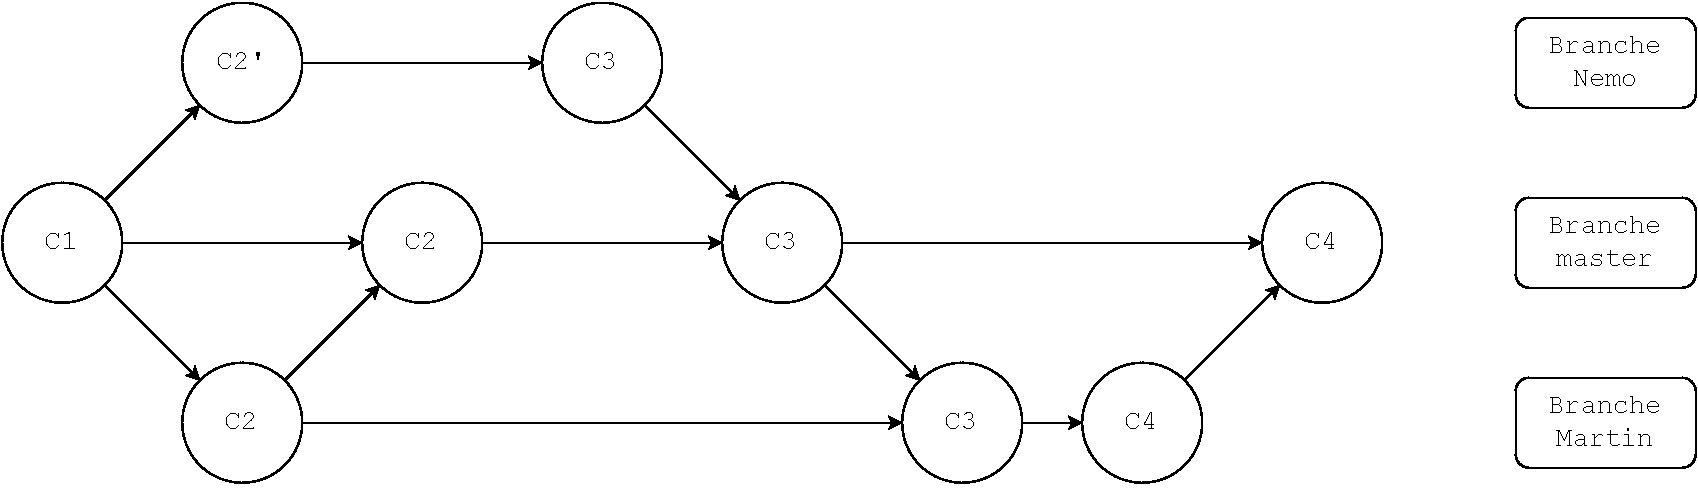
\includegraphics[width=\textwidth]{img/git_branch.pdf}
        \caption{Utilisation de nos 3 branches de git}
        \label{fig:git_branch}
    \end{figure}
\end{center}


% Organisation Code
\subsection{Organisation du code}


\subsubsection*{Problématique}


    Un projet d'une telle envergure nécessite une organisation spéciale afin d'être mené à 
bien. Il s'agit d'une organisation qui doit faciliter l'ajout de nouvelle fonctionnalités,
faciliter la modification de fonctionnalités déjà présente et faciliter la lecture et la 
compréhension de ce qui a déjà été fait.




\subsubsection*{Solutions mises en place}


\subsubsection*{Division en dossiers principaux}


    Sachant que nous nous apprêtions à créer un exécutable pour le projet en lui-même et pour les
tests, nous avons décidé de séparer les sources pour chaque exécutable dans un dossier séparé.


    Ainsi, notre projet est constitué de 4 dossiers principaux: \code{/src}, \code{/tst}, 
\code{/cli\_src}, \code{/evaluator\_src}, comme le schématise le schéma ci-dessous


\begin{center}
    \begin{figure}[H]
        \centering
        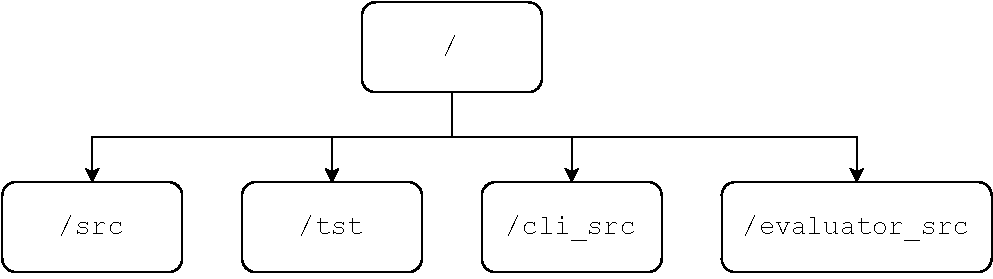
\includegraphics[width=.5\textwidth]{img/main_directories.pdf}
        \caption{Schéma des dossiers principaux du projet}
        \label{fig:main_dirs}
    \end{figure}
\end{center}




\subsubsection*{Division du code par thème}


    Une fois qu'on a divisé en dossiers principaux, on divise le code
dans des sous-dossiers au sein de ces dossiers. Ainsi, on va avoir un
sous-dossier pour les builders et la structure de guilde, un pour les 
tokens et la structure de markets etc... On a aussi un sous-dossier \code{/src/utils},
qui va contenir toutes les structures et fonctions génériques, comme
une structure de file ou une macro \code{MIN} qui retourne le minimum entre 2 entiers.

    L'architecture des sous-dossiers de \code{/src} est schématisé ci-dessous :


\begin{center}
    \begin{figure}[H]
        \centering
        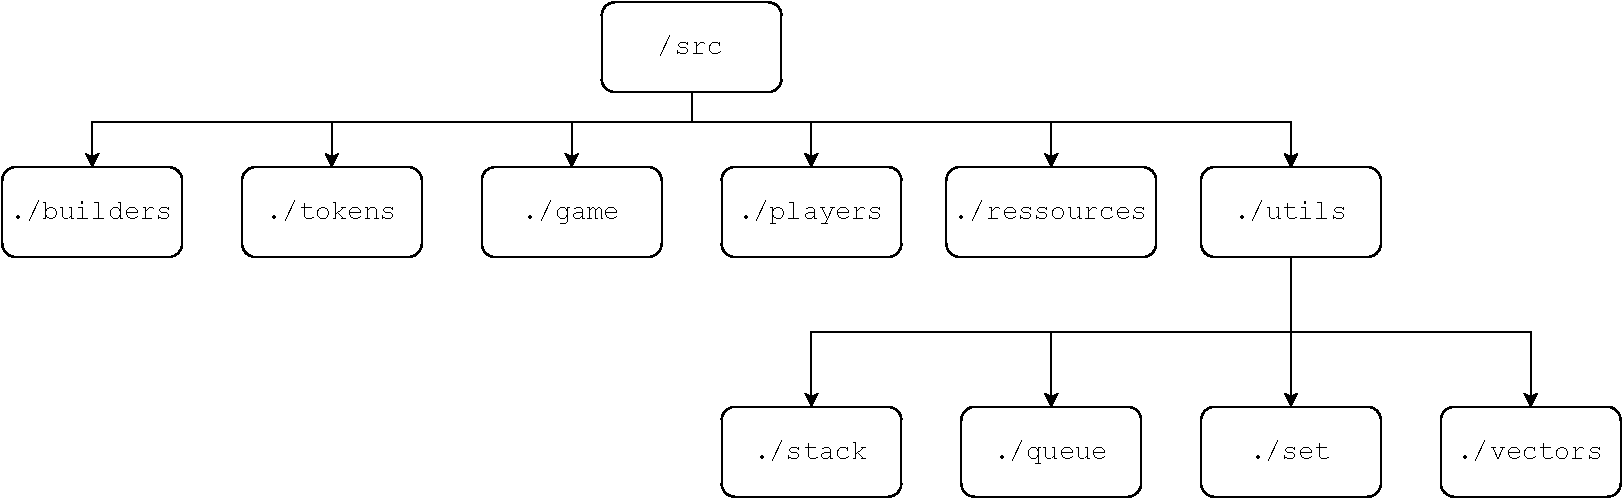
\includegraphics[width=.8\textwidth]{img/src_sub_dir.pdf}
        \caption{Schéma sous-dossiers de $/src$}
        \label{fig:src_sub_dirs}
    \end{figure}
\end{center}




\subsubsection*{Mise en place d'une convention}


\subsubsection*{Problématique}


    Le travail en groupe fait qu'on se retrouve tôt ou tard à lire ou à utiliser des outils codés par une 
autre personne. Ainsi, la forme du code requiert une certaine attention afin de rendre l'utilisation de ces
outils naturelle et la lecture du code uniforme.


\subsubsection*{Solution mis en place}

    Pour résoudre ce problème de forme, on a mit en place une convention de nommage pour les
variables et les fonctions, ainsi que des règles d'écriture. 

    Nous avons décidé d'utiliser la convention \code{snake\_case} pour ce qui est de la forme,
nous nommons les types \lstinline{struct type_t} afin de ne pas les confondre avec d'éventuelles variables.
Une fonction qui devait s'appliquer à un type \lstinline{struct type_t} en particulier est notée
\lstinline{type_function(...)}.

    Vous trouverez ci-dessous des exemples non-exhaustif de la mise en pratique de ces conventions

\begin{lstlisting}[frame=single, caption={Exemples de mise en pratique de ces conventions}]
struct queue_t ;


unsigned int queue_append(struct queue_t* queue, void* value);
\end{lstlisting}




\subsubsection*{Compilation}


\subsubsection*{Problématique}


    Travailler avec telle structure de fichier rend la compilation moins évidente, et fastidieuse si on voulait 
la faire manuellement avec \code{gcc}.


\subsubsection*{Solution mis en place}

    Nous avons utilisé \code{make}, et nous nous sommes appliqué à l'écriture d'un \code{makefile} qui
permettrait d'avancer sereinement dans le projet.

    Notons avant tout que notre \code{makefile} est largement inspiré des ébauches proposées du \href{https://spin.atomicobject.com/makefile-c-projects/}{poste de blog de Job Vranish}, 
ces ébauches formait une fondation solide sur laquelle travailler. Cependant, nous nous sommes tout de même donné le mal de nous l'approprier
afin de l'adapter à notre structure peut-être originale.

    Comme la plupart des sources du dossier \code{/src} sont partagées entre chaque exécutables, nous avons fait le choix de
d'abord chercher tous les fichiers sources de \code{/src}, puis de retirer le fichier \code{/src/projet.c} contenant la fonction main.

\begin{lstlisting}[frame=single, language=sh, caption={Filtrage des fichiers sources du jeu}]
SRC_DIRS := ./src
PROJECT_MAIN_FILE_NAME := ./src/project.c

SRCS := $(shell find $(SRC_DIRS) -name '*.c')
SRCS := $(filter-out $(PROJECT_MAIN_FILE_NAME), $(SRCS))
\end{lstlisting}

    Nous avons opté pour l'utilisation de l'option \code{-Isous\_dossier} de \code{gcc}, permettant de déclarer des librairies systèmes. Ainsi, en 
l'utilisant avec tous les sous-dossiers de \code{/src} et des autres dossiers principaux, cela nous permet de nous limiter à l'écriture de `\lstinline[language=C]{#include "fichier.h"}` dans nos fichiers sources plutôt que le chemin relatif vers le fichier \code{fichier.h}. Étant donné notre arborescence complexe, cela simplifie largement la lecture et l'écriture des dépendances.

    Cependant, il fallait aussi que nos éditeurs, par le biais de clang, puissent être utilisable. D'où l'ajout de la target \code{clang\_custom\_lib\_support} dans
le makefile, permettant de créer le fichier de configuration \code{compile\_flags.txt} indiquant nos librairies systèmes personnalisées à clang.

Finalement l'utilisation d'un nouveau dossier, le dossier \code{/build}. Ce dernier nous sert à stocker tous les fichiers de compilation. Afin de les stocker, nous recréons la structure précédente du fichier, comme le schématise la figure \ref{fig:build_dir}. 

    L'utilisation de ce dossier permet d'avoir une séparation claire entre le reste du projet et la partie compilation.

\begin{center}
    \begin{figure}[H]
        \centering
        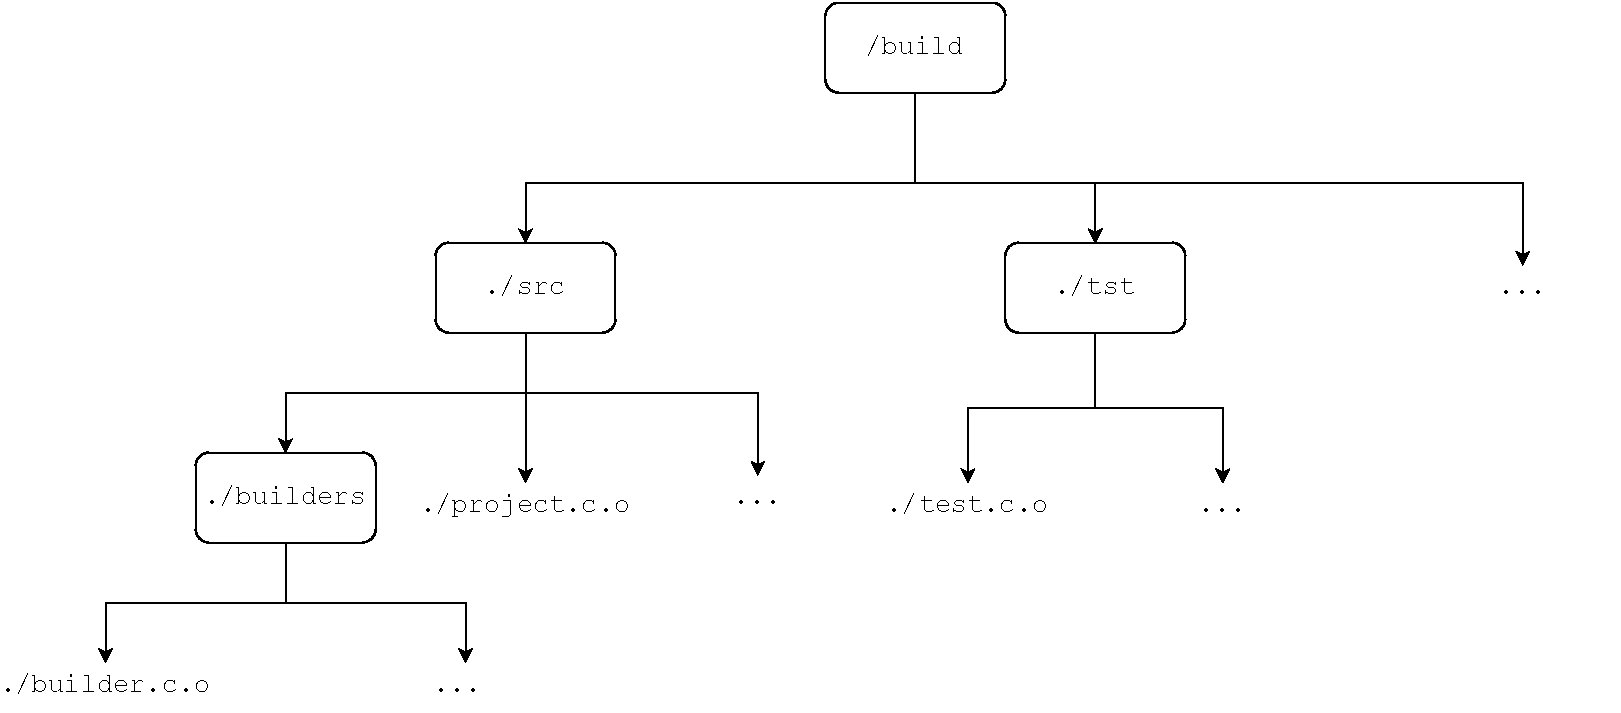
\includegraphics[width=.8\textwidth]{img/build_dir.pdf}
        \caption{Schéma arboressence du dossier /build}
        \label{fig:build_dir}
    \end{figure}
\end{center}





\section{Présentation du projet}


\subsection{Le splendor}

Le splendor est un jeu de société se jouant en tour par tour, mettant en jeu des jetons de couleurs, des architectes, et dont le but est d'obtenir le plus de points possibles. Les jetons apportent des ressources permettant ensuite de recruter des architectes. Les architectes, quant à eux, permettent de générer des ressources à chaque tours et rapportent des points.

Les architectes sont stockés dans une guilde, et sont disponibles par niveaux. Pour chacun des niveaux, seuls un nombre prédéterminé sont disponible. Lors de l'achat d'un architecte, on le remplace par le prochain disponible de la pile du niveau associé, comme le schématise la figure \ref{fig:buy_builder} suivante : 

\begin{figure}[H]
    \centering
    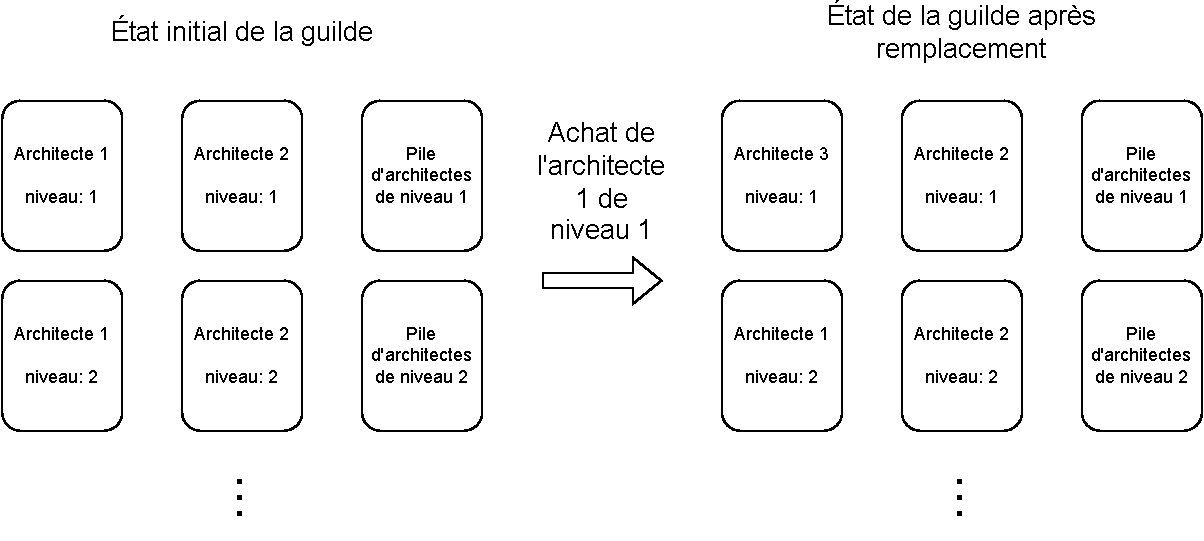
\includegraphics[width=.8\textwidth]{img/guild.pdf}
    \caption{Schéma de l'achat et remplacement d'un architecte de niveau 1}
    \label{fig:buy_builder}
\end{figure}

Les jetons sont eux stockés dans un marché et sont disposés sur un plateau carré. Pour être récupérés, les jetons doivent être pris connexes par rapport au chemin.


\begin{figure}[H]
    \begin{minipage}[c]{0.45\textwidth}
        \centering
        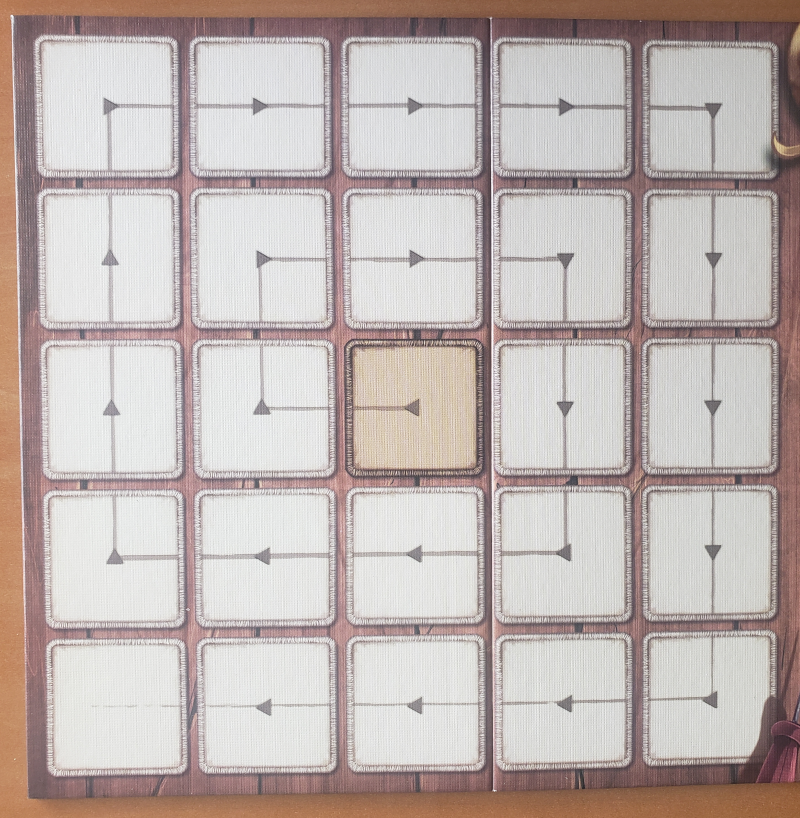
\includegraphics[width=\textwidth]{img/projMunificenceBoard.png}
    \end{minipage}
    \hfill
    \begin{minipage}[c]{0.45\textwidth}
        \centering
        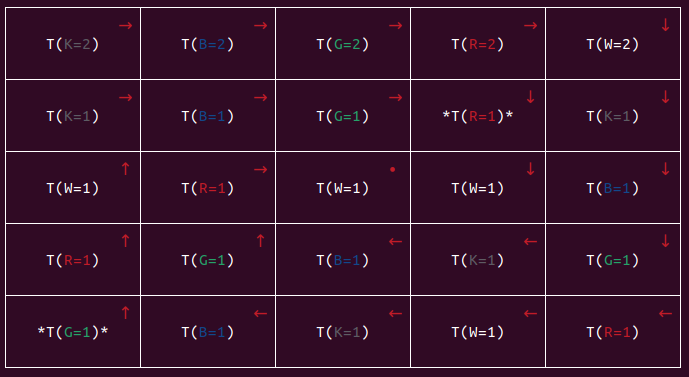
\includegraphics[width=\textwidth]{img/board-terminal.png}
    \end{minipage}
    \caption{Images schématisant le plateau et le chemin reliant les jetons}
    \label{fig:board_example}
\end{figure}

À chaque tours, il n'est possible de faire qu'une action, on peut choisir de soit prendre entre 1 et 3 jetons dans le marché, soit d'embaucher un architecte auprès de la guilde. Lors de la prise de jetons ou de l'embauche d'un architecte, il est possible qu'un pouvoir soit attaché à ce dernier, et alors le pouvoir s'exécute à la fin de l'action.

\begin{summary}
Au début d'un tour, il est aussi possible, si on a accumulé une faveur, de l'utiliser pour prendre un jeton dans le marché ou pour renouveler les architectes disponibles d'un niveau donné de la guilde.
\end{summary}


\subsection{Contraintes du projet}

En plus de devoir implémenter, nous devions faire attention aux contraintes suivantes du sujet :

\begin{itemize}
    \item Ne pas modifier les fichiers \code{color.h}, \code{builder.h} et \code{token.h} qui étaient fourni.
    \item Utiliser exclusivement le langage C.
    \item Le fichier \code{makefile} devait définir une règle \code{project}, qui devait créer l'exécutable nommé \code{project} à la racine du projet, et la règle \code{all} devait faire appel à la règle \code{project}.
    \item Le fichier \code{makefile} devait aussi définir une règle \code{test}, qui devait exécuter les différents tests du projet.
    \item La définition de \code{NUM\_LEVELS} et \code{NUM\_TOKENS} doit être possible lors de l'appel de la règle \code{project}
\end{itemize}




\subsection{Nos contraintes}
\label{nomalloc}

A titre d'expérimentation, nous nous sommes aussi contraint à ne pas utiliser de \code{malloc}.

Le code sera entièrement écrit en anglais et on privilégiera l'utilisation de pointeur dans les paramètres de nos fonctions. 




\input{parties/Implementation/Implémentation}

\section{Tests}
\label{tests}

\subsection*{Problématique}

Lorsque que le code est important et est amené a évoluer avec de nouvelles fonctionnalités, il peut devenir intéressant de tester le comportement des fonctions pour vérifier qu'elles respectent des règles de base. Dans notre cas de figure nous testons une grande majorité des fonctions de base, les autres fonctions découlant de ces dernières.

\subsection{Mise en place des tests}

Tout comme le reste du code, les tests sont séparés en sous dossiers par thème. Chaque thème possède une fonction qui regroupe les tests des fonctions associées à ce thème, qui sont alors exécutés par l'exécutable de test.


\begin{lstlisting}[frame=single, caption={Exécution des tests}]
int main(int argc, char *argv[])
{
	test_token();
	test_builders();
	test_market();
	test_guild();
	test_players();
	test_utils();
	test_skills();
 
	return EXIT_SUCCESS;
}
\end{lstlisting}

\subsection{Vérifications effectuées}

Chaque tests vérifie le comportement attendu de la fonction, et si elle respecte les règles définies en amont. Dans cet exemple on vérifie si l'initialisation d'un joueur créer bien un joueur vide.

\begin{lstlisting}[frame=single, caption={Test init player}]
int test_init_players()
{
	struct player_t new_player = init_player();

	if(player_get_points(&new_player) != 0)
	{
		/* Error message */
		return 0;
	}

	struct ressources_t* player_ressources = player_get_ressources(&new_player);
	
	for (int index = 0 ; index < MAX_BUILDERS ; ++index)
	{
		if (player_ressources->guild.builders[index]) 
		{
			/* Error message */
			return 0;
		}
	}

	for (int index = 0 ; index < NUM_TOKENS ; ++index)
	{
		if (player_ressources->market.tokens[index]) 
		{
			/* Error message */
			return 0;
		}
	}
	return 1;
}
\end{lstlisting}


\section{Solutions algorithmiques}

\subsection{Récupérer des jetons connexes d'un marché}
\label{linkedtokens}

Pour récupérer nb-jetons connexes d'un marché, on parcourt ce dernier du début à la fin avec un compteur de jetons connexes.

\noindent Différents cas de figure :
\begin{itemize}
    \item Si le pointeur n'est pas \code{NULL} (la case du marché contient un jeton) :
    \begin{itemize}
        \item Si le compteur est égal à nb alors on ajoute l'indice à une liste sans incrémenter le compteur.
        \item Sinon on incrémente le compteur de 1
    \end{itemize}
    \item Si le pointeur est \code{NULL} (la case du marché est vide) :
    \begin{itemize}
        \item On remet le compteur à 0.
    \end{itemize}
\end{itemize}

Ainsi à l'issue de la boucle on peut retourner un indice présent dans la liste pris de manière aléatoire. Si la liste est vide, on retourne -1.

La complexité de cet algorithme est $\theta(n)$, avec n le nombre de jetons dans la partie.

\begin{summary}
Ici on considère des jetons connexes lorsqu'ils sont reliés par le chemin continu dessiné par le plateau (cf \ref{fig:board_example}) et non lorsqu'ils sont voisins sur le plateau. C'est un choix assumé.
\end{summary}








\section{Difficultés de mise en oeuvre}


\subsection{Implémentation des pouvoirs}

Il y a plusieurs manières de mettre en place les pouvoirs, qui ont chacune des avantages et des inconvénients.

\subsubsection*{Implémentation avec un switch}

Comme présenté précédemment (cf. \ref{skills}), nous avons décidé de les implémenter à l'aide de pointeurs de fonctions, comme proposé dans le sujet. Cependant, une implémentation possible des pouvoirs aurait pu être l'utilisation du type \code{enum skill\_id} et utiliser un \code{switch} dans la fonction exécutant le tour d'un joueur. Ainsi la fonction \code{skill\_exec} ressemblerait à quelque chose comme suivant : 

\begin{lstlisting}[language=c, frame=single, caption={Pseudocode de la version possible de skill\_exec avec un switch}]
enum skill_ids {SKILL_1, SKILL_2, ...}

skill_exec(skill_id)
{
    switch (skill_id)
    {
        case SKILL_1:
            /* Execute SKILL_1 */

        case SKILL_2:
            /* Execute SKILL_2 */
            
        ...
    }
}
\end{lstlisting}

Cela aurait eu comme avantage le fait de pouvoir avoir une exécution personnalisée de chaque pouvoirs. Ainsi, si un pouvoir nécessite de demander au joueur un des informations supplémentaires, comme la cible du pouvoir, cela est faisable.

Le problème de cette implémentation, c'est que l'ajout de nouveaux pouvoirs est fastidieux, et nécessite la modification de la fonction exécutant les pouvoirs \code{skill\_exec}, on se retrouve pour un pouvoir donné avec une division de la localité de la logique de l'exécution de ce dernier, ce qui n'est pas idéal pour la maintenabilité du code.


\subsubsection*{Implémentation avec des pointeurs de fonctions}

De l'autre côté, l'utilisation de pointeurs de fonctions permet de facilement créer de nouveaux pouvoirs et de les ajouter dans le jeu. On a juste à ajouter le nouveau pouvoir dans le tableau les contenant tous, et à ajouter un identifiant pour ce pouvoir, car la fonction \code{skill\_exec} se réduit globalement à ce quit suit :


\begin{lstlisting}[language=c, frame=single, caption={Pseudocode de la version de skill\_exec avec des pointeurs de fonction}]
enum skill_id {SKILL_1, SKILL_2, ...}

skill_exec(skill_id)
{
    skills[skill_id](args);
}
\end{lstlisting}


La contrainte que cela impose est que tous les pouvoirs doivent avoir la même signature. Ainsi, si certains pouvoirs doivent avoir accès à plus d'informations que d'autres, la signature des pouvoirs doit le permettre.

Pour créer une telle signature, encore une fois, plusieurs options sont possible. La première serait de dire qu'on passe en paramètre une union de types, avec chaque type qui serait associé à un pouvoir, décrivant les données nécessaire à son exécution. Même si ça semble bien fonctionner sur le papier, pour créer l'argument à passer en paramètre, il faut passer par un \code{switch} ou quelque chose de similaire nous ramenant au cas de l'implémentation précédente.

Nous avons donc au final opté pour passer en paramètre 2 arguments, le tour courant et ce qui a déclenché le pouvoir. Cela restreint légèrement les possibilités des pouvoirs, et nous avons du nous résoudre à limiter certains d'entre eux, ils ont pour certains un comportement aléatoire, c'est-à-dire que lorsqu'il est question de voler un jeton, on ne laisse pas le choix au joueur et on en prend un au hasard.

Dans le cadre de nos joueurs ayant un comportement de toute façon aléatoire, ceci ne pose pas problème, mais il est normal de vouloir que le joueur puisse avoir le choix, surtout si on décidait d'intégrer des stratégies à nos joueurs ou de faire jouer des humains.

\subsubsection*{Amélioration possible}

Ainsi, nous avons imaginé, sans avoir pris le temps de l'implémenter, qu'associer à chaque pouvoir un "pre-pouvoirs", une fonction se chargeant de demander aux joueurs les arguments nécessaire au bon fonctionnement du pouvoir. Ainsi, en ayant la fonction \code{execute\_skill}, n'aurait qu'a exécuter le "pre-pouvoir" puis le pouvoir associé à \code{skill\_id}. Cette implémentation permettrait, pour ajouter un pouvoir, de n'avoir qu'à ajouter la fonction pouvoir et la fonction "pre-pouvoir" et à les rajouter dans un tableau.


\begin{lstlisting}[language=c, frame=single, caption={Pseudocode de la version de skill\_exec avec les "pre-pouvoirs"}]
enum skills_id {SKILL_1, SKILL_2, ...}

skill_exec(skill_id, args)
{
    void* custom_args = preskill[skill_id](args);
    skills[skill_id](args, custom_args);
}
\end{lstlisting}







\subsection{Stockage des architectes et des jetons}

\subsubsection*{Problème}

Les architectes, les jetons  et les associations de pouvoirs sont générés puis stockés en statique dans \code{builder.c}, \code{token.c} et \code{skills.c}, durant le reste de la partie on utilise seulement les pointeurs et les méthodes de ces derniers. L'avantage est que l'on a pas besoin de connaître l'implémentation de la structure pour pouvoir interagir avec.

Cela pose un problème, ne connaissant pas l'architecture de ces structures en dehors de où elles sont créées, il nous est impossible de générer plusieurs decks en parallèle ou de les stocker ailleurs. Dans notre cas de figure cela signifie qu'on ne peut stocker les jetons et les architectes dans notre structure de partie. On ne peut donc pas jouer 2 parties, puis afficher la première. 

\subsubsection*{Solutions envisagées}

La solution la plus simple serait de rendre public la structure d'architecte pour pouvoir les stocker la structure de partie. Mais cela nous est impossible à cause des caractéristiques du sujet.

La solution retenue est de devoir régénérer les architectes, les jetons et les pouvoirs à partir des paramètres (graines) de la partie avant d'afficher ou de modifier une partie différente.




\section{Évaluation de parties}

%label pour referencement
\label{evaluator}

\subsection*{Problématique}

Maintenant que nous sommes capable de jouer des parties de manières indépendantes, il est intéressant de trouver quel couple de graine donne lieu aux parties les plus viables. Pour cela nous avons besoin d'avoir accès aux statistiques de la partie et de jouer un grand nombre de parties avec des graines différentes.

\subsection{Extraction des statistiques d'une partie}

Lorsque qu'un tour est joué, on retourne les statistiques de ce dernier à travers la structure \code{turn\_statistics} qui est ensuite ajouté aux statisques globales de la partie au travers de la structure \code{game\_statistics}.

\begin{lstlisting}[frame=single, caption={Structures pour récupérer les statistiques}]
struct turn_statistics
{
	enum choice choice;
	int used_favor;
	int used_skill;
	int num_picked_tokens;
	int forced_skip;
};


struct game_statistics
{
	int choices[NUM_CHOICE];
	int used_favor;
	int used_skill;
	int num_picked_tokens;
	int forced_skip;
	int nb_turns;
	int result; 
};
\end{lstlisting}

\subsection{Test d'un grand nombre de parties}

Maintenant que l'on peut récupérer les statistiques d'une partie, on teste chaque couple de graines avec 100 graines aléatoires (\code{random\_seed}) pour récupérer une moyenne des statistiques pour chaque couple que l'on affiche dans la sortie standard sous la forme d'un csv. On peut alors récupérer ces données dans un fichier pour les analyser.

\begin{lstlisting}[frame=single, caption={Affichage des résultats}]
seed_builders;seed_token;choices;used_favor;used_skill;num_picked_tokens;forced_skip;nb_turns;result
1;0;1.85,6.26,1.12;1.27;1.58;12.37;0.01;9.23;0.48
2;0;1.08,7.33,1.10;0.99;1.76;14.23;0.13;9.51;0.35
3;0;1.39,6.66,1.08;0.98;1.22;13.16;0.07;9.13;0.42
4;0;1.47,6.60,1.05;0.98;1.36;13.19;0.05;9.12;0.43
5;0;1.32,6.29,0.96;0.92;1.85;12.11;0.03;8.57;0.53
6;0;1.48,6.74,1.08;0.96;1.04;13.22;0.04;9.30;0.35
7;0;1.84,6.11,1.01;0.97;2.57;12.06;0.02;8.96;0.60
8;0;1.14,6.62,1.06;0.97;1.60;13.03;0.03;8.82;0.55
9;0;1.67,6.57,1.01;0.96;1.23;13.03;0.04;9.25;0.43
...
\end{lstlisting}

\subsection{Analyse des résultats}

A l'aide d'un programme écrit en \code{Python}, on peut visualiser l'influence des différentes graines sur différents paramètres.


\begin{figure}[H]
   \begin{subfigure}[b]{0.3\textwidth}
        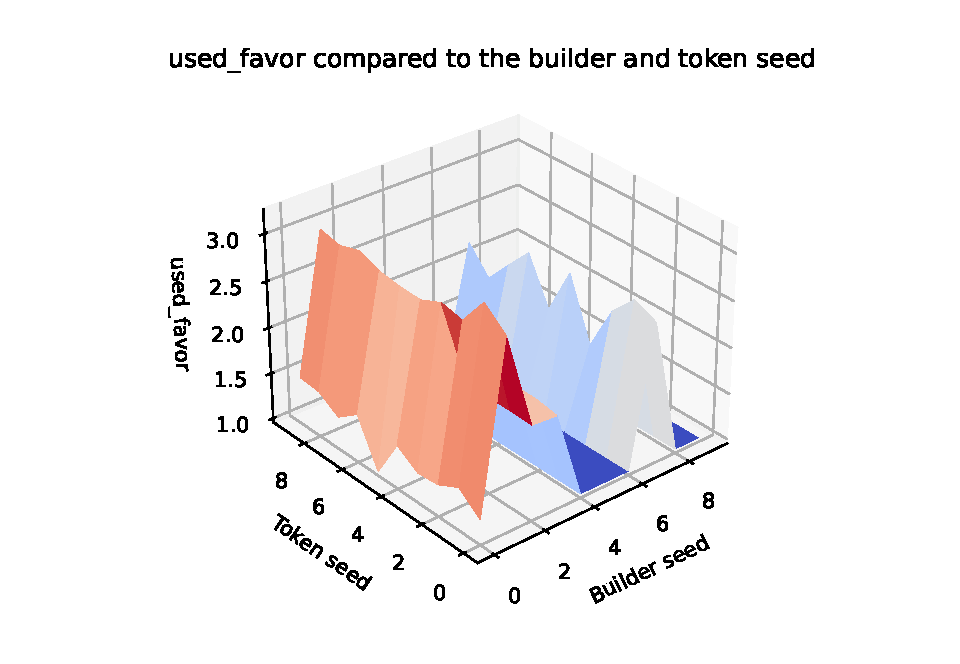
\includegraphics[width=\textwidth]{img/favor.pdf}
    \end{subfigure}
    \begin{subfigure}[b]{0.3\textwidth}
        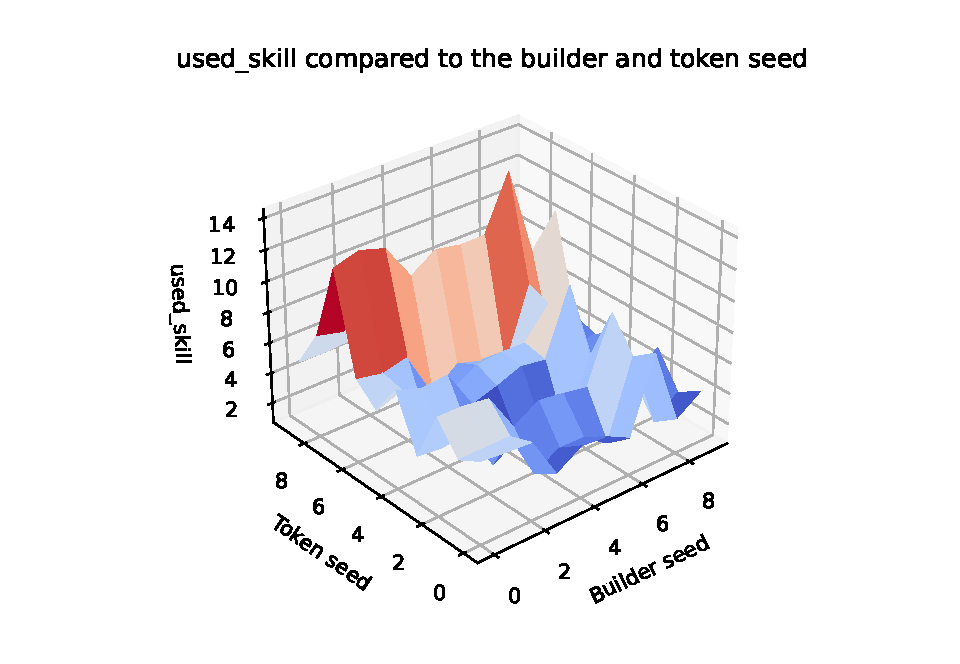
\includegraphics[width=\textwidth]{img/skills.pdf}
    \end{subfigure}
    \begin{subfigure}[b]{0.3\textwidth}
        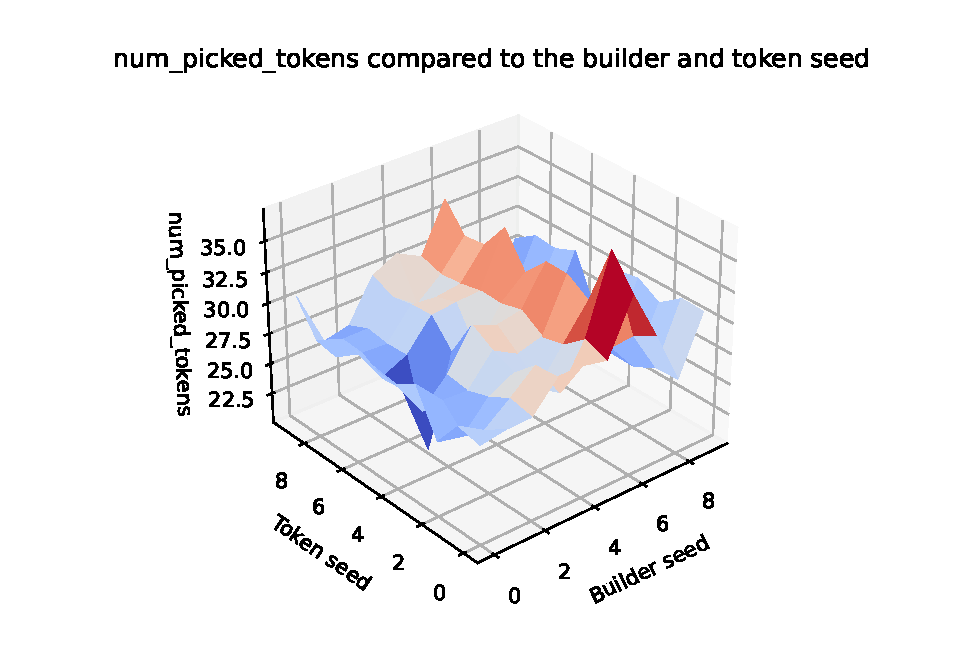
\includegraphics[width=\textwidth]{img/tokens.pdf}
    \end{subfigure} 
    \\
    \begin{subfigure}[b]{0.3\textwidth}
        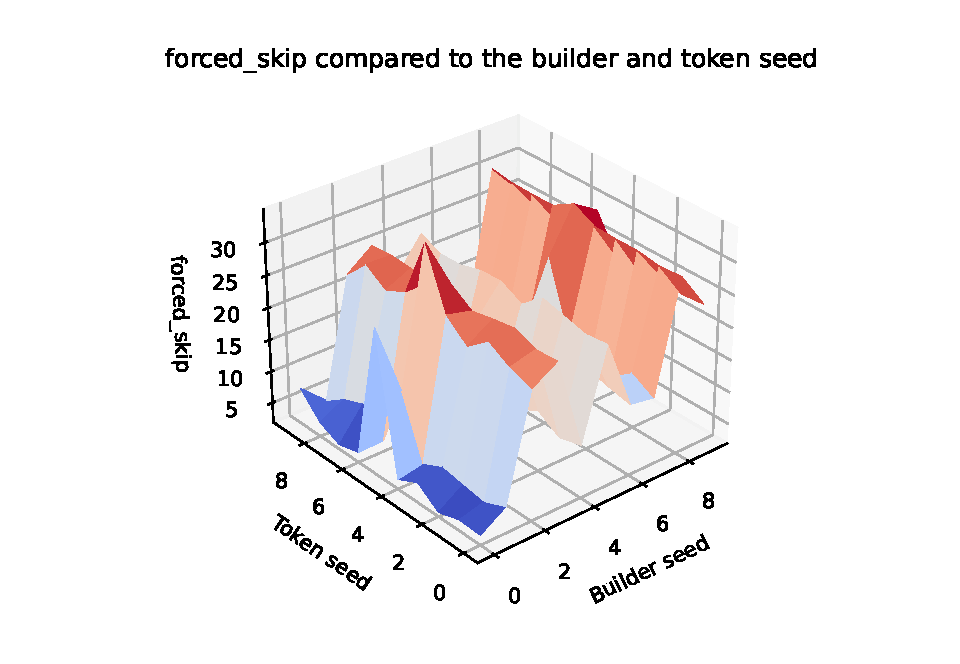
\includegraphics[width=\textwidth]{img/skip.pdf}
    \end{subfigure}
    \begin{subfigure}[b]{0.3\textwidth}
        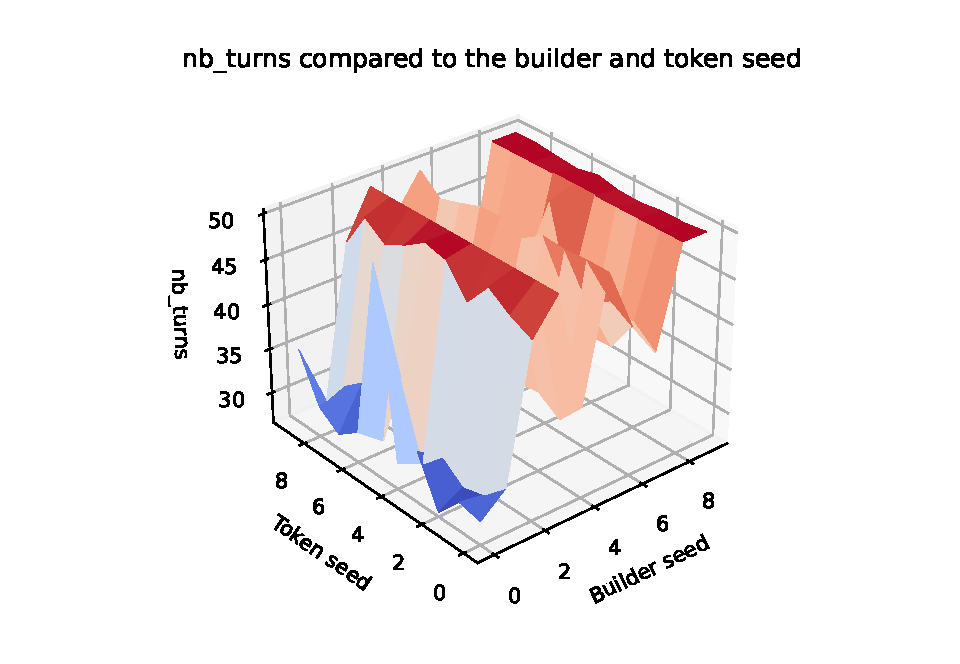
\includegraphics[width=\textwidth]{img/turns.pdf}
    \end{subfigure}
    \begin{subfigure}[b]{0.3\textwidth}
        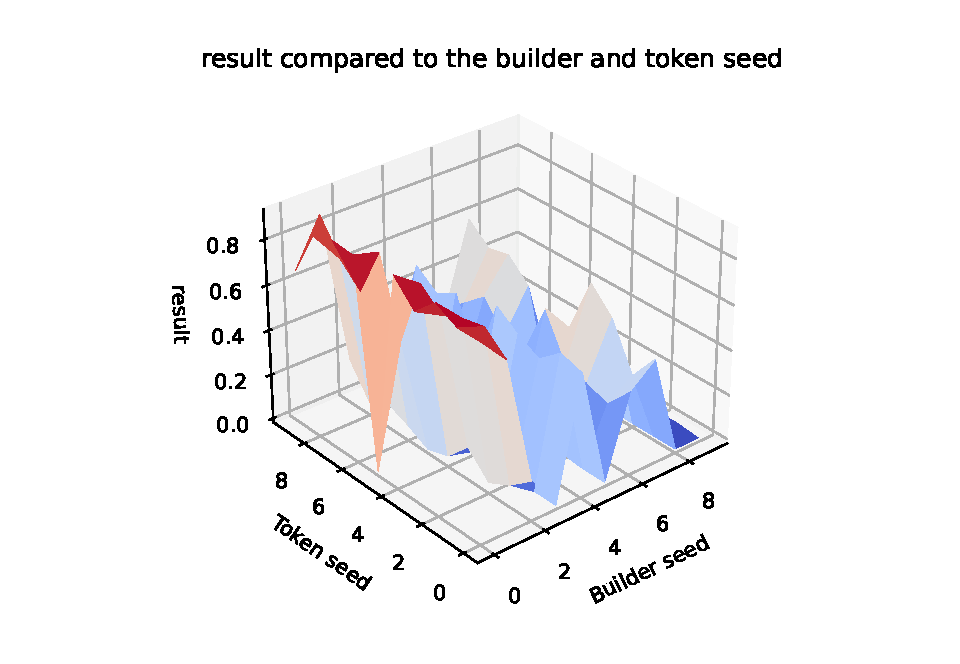
\includegraphics[width=\textwidth]{img/result.pdf}
    \end{subfigure} 
    \caption{Influence des graines sur différents paramètres de la partie}
\end{figure}
\begin{summary}
\textbf{Précision} : la graine 0 n'est pas générée aléatoirement mais correspond à un deck généré à la main afin d'avoir un jeu équilibré (selon nous).
\end{summary}
A partir de ces graphiques, on remarque un comportement intéressant : la graine des architectes a beaucoup plus d'influence sur la viabilité de la partie (beaucoup de tour et pas trop de tour passés) que celle des jetons. Par exemple on voit que les joueurs sont forcés à passer souvent leur tour avec la graine d'architecte n°3 car il y a seulement 2 architectes générés dans cette dernière.
\label{cli}



\section*{Conclusion}
\addcontentsline{toc}{section}{Conclusion}




\end{document}